\chapter{Complete examples of \SBGNERLone maps}

The following maps present complete examples of SBGN \ERs representing biological processes. They by no mean exhaust the possibilities of  \SBGNERLone.\\

\fig{PCR} presents the different relations between the four entities involved in a Polymerase Chain Reaction (PCR). This examplifies the use of the \glyph{entity}, the logical operator \glyph{or}, the \glyph{state variable} ``existence'', the \glyph{unit of information}, as well as the relationships \glyph{interaction}, \glyph{assignment}, \glyph{necessary stimulation} and \glyph{absolute inhibition}.

\begin{figure}[htb]
\begin{center}
\scalebox{0.5}{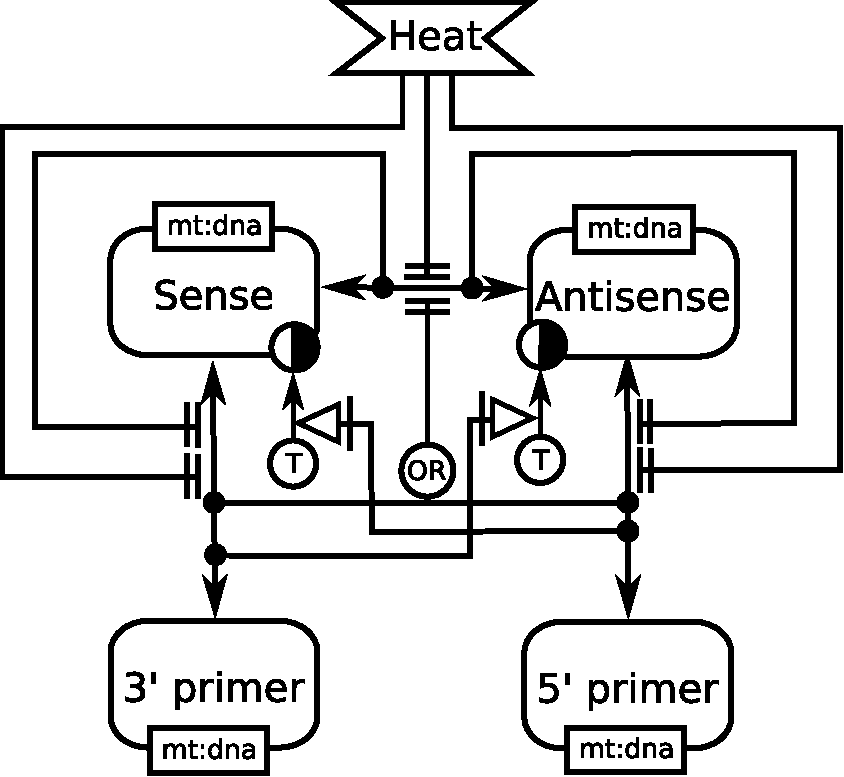
\includegraphics{examples/PCR}}
\caption{Principle of the Polymerase Chain Reaction.}\label{fig:PCR}
\end{center}
\end{figure}

\fig{CaMKII} depicts the effect of a depolarisation (dV) on the intracellular calcium, that binds to calmodulin, that itself binds to the calcium/calmoduline kinase II (CaMKII). The binding of calmodulin inhibits the folding of CaMKII monomer on itself, thus relieving the inhibition on the kinase activity. The phosphorylation of the glutamate receptors finally leads to the Long Term Potentiation (LTP) of the synapses. In addition, the map shows the effect of trans-phosphorylation on threonine 286, that makes the enzyme constitutively active, and on threonine 306, that renders the kinase insensitive to calmodulin, as well as the dimerisation of the kinase.

\begin{figure}[H]
  \centering
  \vspace*{-0.75em}
  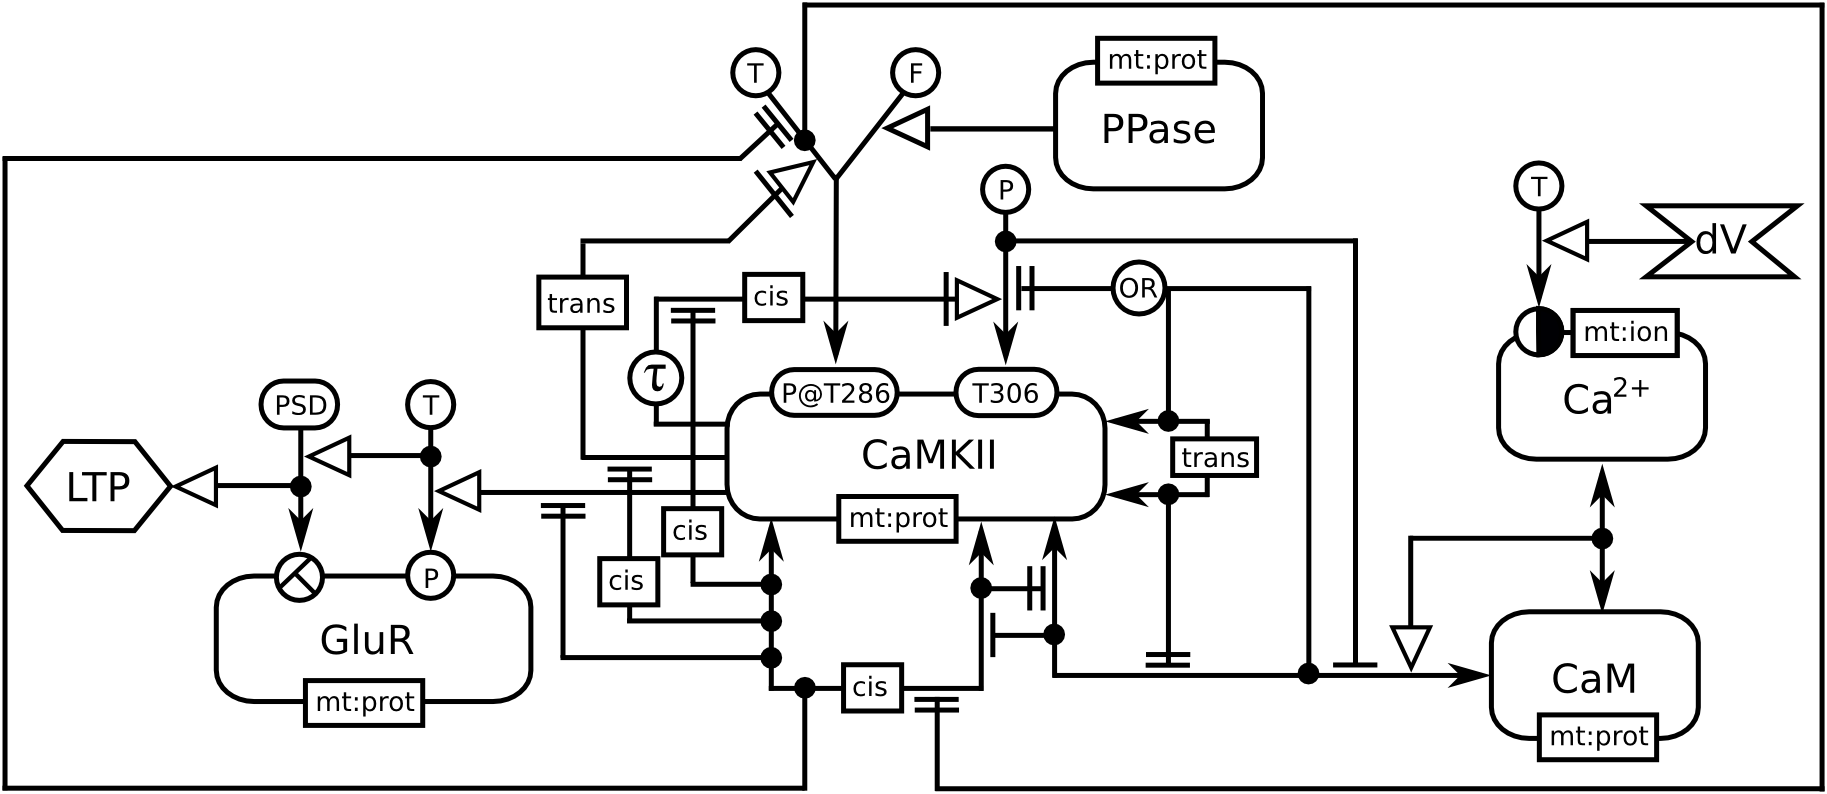
\includegraphics[scale=0.45]{examples/CaMKII-intro}
   \caption{Regulation of calcium/calmoduline kinase II effect on synaptic plasticity.}
  \label{fig:CaMKII}
\end{figure}